\documentclass[a4paper]{article}
\usepackage[english]{babel}
\usepackage{enumerate}
\usepackage{amsmath}
\usepackage{tikz}
\usepackage{graphicx}

\begin{document}

% custom commands to make matrices more convenient
\newcommand{\bvect}[1] {\begin{bmatrix} #1 \end{bmatrix}}
\newcommand{\pvect}[1] {\begin{pmatrix} #1 \end{pmatrix}}

\title{Designing a Dynamic Kick for the Nao Robot}
\author{ Inge Becht \\ 
         Maarten de Jonge \\ 
         Richard Pronk \\\\
         \large{University of Amsterdam}}
\date{\today}
\maketitle

\section{Introduction} 
Our research is concerned with making a dynamic, closed
loop kick for the Nao robot. The Nao is a humanoid robot made by
Aldebaran Robots\footnote{http://www.aldebaran-robotics.com/en/}. It is used in
the Stand Platform League of the
Robocup\footnote{http://wiki.robocup.org/wiki/Standard\_Platform\_League}, an organisation which organizes football (soccer)
competitions for autonomous robots.

Kicking, of course, is an important part of football, and thus a good kick is vital to achieving good results in the Robocup. There are essentially two ways of making a humanoid robot kick a ball:
\begin{enumerate}
  \item Positioning the robot in a specific place relative to the ball, then executing a manually specified series of movements
  \item Using the location of the ball, and the angle you want the ball to go to dynamically determine a trajectory for the robot to move
\end{enumerate}
The first one is referred to as a \emph{keyframe motion}, while the second one is the subject of this paper.

\section{Basic information about the Nao}
The Nao is a 58 cm high humanoid robot developed by Aldebaran Robotics. The Nao
is equipped with all kinds of different gadgets. Here we will discuss the most
important ones 
\begin{itemize}
    \item foot sensors
    \item space
    \item rotations
    \item length of end effectors
    \item built in functions
    \item Terminalogy
\end{itemize}


\section{Motivation for this project} 
While the Dutch Nao Team (the team that represents the Netherlands in the Standard Platform League of the Robocup) has achieved some degree of success with simple keyframe motions, they are clearly not optimal; a lot of time is wasted positioning the robot at just the right angle relative to kick the ball towards the goal. Furthermore, if the ball gets moved after the kicking motion has started, it's impossible for the robot to correct its kicking path. These are all problems that can be reduced with a dynamically generated motion, which is why we will attempt to create one. If we succeed in our endeavour, the resulting kick will be integrated in the Dutch Nao Team's codebase.

\subsection{Stability}
Since there is more than one player on
the field  chasing after the ball,
there is lots of interference from other Naos while kicking. Due to the
instability of the Nao this results in falling down quite often, even more
so when there is no compensation for it when executing a motion. A dynamic
kick keeps track of the stability and will execute a kick that keeps the Nao
most stable.

Overheating is also a problem for Naos. When this occurs the joints will perform
not as expected or even fail. Using this dynamic system the temperature of the
joints can be used to prevent overheating. The executed kick will depend less
on force so the robot will spare its joints.

\subsection{Harder kicks and better stability}
Being able to define when a kick is stable enough to execute we can make a
trade-off between how far the ball is kicked and the stableness of the
robot, resulting in harder kicks then when using keyframe motions.

\subsection{Helping the Dutch Nao Team}
 Working on this project will help the Dutch Nao Team in their competition. The
current keyframe motion used by DNT is very brittle, with our dynamic kick we will create a
more robust kick that can give our universities team a bigger chance of
winning in competitions. 
This integration makes this project a valuable activity in the long run, and not
just a one time experiment.

\section{Methodology}
The task of kicking a ball requires a couple of things: We need to find a path
for the foot to travel, then we need a way to calculate the joint angles
corresponding to the required position of the foot (inverse kinematics), and all
the while we have to make sure the robot doesn't fall over.

\subsection{Automatic balancing during the kicking motion}
The Nao should be balanced during its kick, regardless of the motion of the
kicking leg. For this a center of mass-based approach is used along with a
proportional controller (\emph{cite wikipedia or something here}).

\subsubsection{Center of mass and support polygon}
This balancing approach requires knowledge of 2 concepts; the \emph{center of mass},
and the \emph{support polygon}. The center of mass (\emph{CoM}) is the weighted average
location of the Nao’s mass, while the support polygon is the location on the
floor over which the center of mass must be located to achieve stability. In the
case of a robot standing on the ground, the support polygon is the convex hull
of the feet touching the ground. Because the CoM is only used in conjuction with
a proportional controller (which only requires a single target point) and the
robot will only be balancing on one foot, the support polygon can be simplified
to be a single point slightly in front of the location of the support leg's ankle
joint.

The center of mass is a bit more complex to calculate. It's defined as the sum
of each component’s \emph{centroid} (its own center of mass) multiplied by its
mass, divided by the total weight (equation \ref{eq:CoM}). This of course
requires each centroid to be described in the same coordinate system.
\begin{align}
  \frac{\sum_i \vec{c}_i m_i} {m}        \label{eq:CoM}
\end{align}
In the Nao’s documentation, each component’s centroid is described relative to
its own coordinate system, and offsets are included to convert between adjacent
components’ coordinate systems. To handle this, we construct a chain of
transformations to walk through each component while calculating the center of
mass of the entire robot.

\subsubsection{The proportional controller}
The goal of the proportional controller (\emph{P-controller}) is to keep the
CoM as close as possible to the center of the support polygon at all times.
The CoM is calculated relative to the standing leg's ankle joint, and we define
the center of the support polygon to be ``about 3cm in front of that''. Thus the
error-calculation becomes:
\begin{align}
  d &= \begin{bmatrix} 3 \\ 0 \end{bmatrix} - \vec{CoM_{xy}} \\
  error &= \sum_{i \in d} |i|
\end{align}
The Z-axis is ignored, because the height is irrelevant in this case (the CoM
balancer only accounts for gravity, not other phenomena such as momentum).

The proportional control equation with an arbitrary \emph{gain} parameter is
shown in equation \ref{eq:pcontrol}.
\begin{align}
  P_{out} = gain * error        \label{eq:pcontrol}
\end{align}

Actuation is achieved solely through the hip's pitch and roll of the standing leg.
The rotation angles are obtained by searching through all combinations of the angles
$(0, P_{out}, -P_{out})$ (e.g. $(pitch = 0, roll = 0)$, $(pitch = 0, roll = P_out)$, etc)
for both joints (thus searching through a $3^2$ sized space) and selecting the pair
of angles with the largest reduction in error. This approach is acceptably fast
when actuating two joints, but has the downside of having a complexity of $\mathcal{O}(3^n)$
in amount of actuated joints.

\newpage
\section{Using force-sensitive resistors to keep balance}

As the balacing using the Center Of Mass allows a good conversion to a stable position it does not react to external influences.
Using the force-sensitive resistors under Nao's feet these external influences can be measured and neutralized.
\begin{figure}[htb]
	\centering
	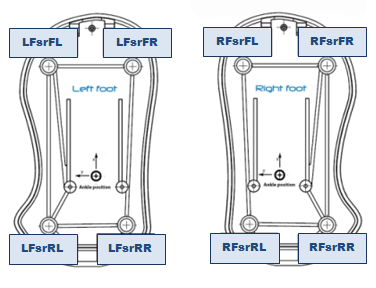
\includegraphics[scale=0.75]{pics/naosfeet.jpg}
	\label{fig:fsr_plot}
	\caption{The force-sensitive resistors under Nao's feet}
\end{figure}\\
While kicking a ball you stand on one leg while kicking with the other leg, the leg on which the robot stands is called the support leg. 
When taking the left foot as support leg (the same goes for the right leg), the foot will be divided into four sections (Front, Left, Right and Back). 
\begin{itemize}
    \item $Front_t = (1-s) * Front_{t-1} + s * (LFsrFL + LFsrFR)$
    \item $Left_t = (1-s) * Left_{t-1} + s *(LFsrFL + LFsrRL)$
    \item $Right_t = (1-s) * Right_{t-1} + s *(LFsrFR + LFsrRR)$
    \item $Back_t = (1-s) * Back_{t-1} + s *(LFsrRL + LFsrRR)$ 
\end{itemize}
Where s is the smoothing parameter and t is the present time.

\subsection{proportional-Derivative controller}

The Proportional-Derivative controller (PD-controller) is a special case of the Proportional-Integral-Derivative controller (PID controller) where the integral term (I) is not used.  The PD-controller has 2 terms the proportional (P) and the derivative (D) term. The response of each term can be tweaked using there own tweaking parameter, the proportional gain $K_p$ and the derivative gain $K_d$. \\
The proportional term is given by:
\[
P_{out}  = K_pe(t)
 \]
and the derivative term is given by:
\[
D_{out}  = K_d\frac{d}{dt}e(t)
\]
The Hip Pitch is used to compensate for the error in the x direction (Front and Back) while the Hip Roll compensates for the error in the y direction (Right and Left).
The angle offsets for the hip joints are calculated by;
\begin{itemize}
    \item $P_{out} x = (Front_t - Back_t) * K_p$
    \item $P_{out} y = (Right_t - Left_t) * K_p$
    \item $D_{out} x = \frac{Front_t - Back_t}{timeTaken}K_d$
    \item $D_{out} y = \frac{Right_t - Left_t}{timeTaken}K_d$
    \item  $Offset$ $Hip$ $Pitch$ $= P_{out}x + D_{out}x$ 
    \item $Offset$ $Hip$ $Roll$ $=  P_{out}y + D_{out}y$ 
\end{itemize}
Where $timeTaken = time_t - time_{t-1}$(the time taken between the current and previous execution) .\\\\
Using an error band to allow a range of stable points and therefore better conversion. Without this range the robot would diverge and finally fall due to the oscillation. When the error is within this range it will be set to 0, this allows the robot to converge to a stable position. Due to the robots build the forward and sideways stabilization act differently, different error bands are therefore needed. The function of the proportional term becomes;
\[
  P_{out}x = \left\{ 
  \begin{array}{l l}
     (Front_t - Back_t)K_p& \quad \text{if $Thres_{min X} < (Front_t - Back_t) < Thres_{max X}$}\\ 
     0& \quad \text{Otherwise}\\
  \end{array} \right.
\]
\[
  P_{out}y = \left\{ 
  \begin{array}{l l}
     (Right_t - Left_t)K_p& \quad \text{if $Thres_{min Y} < (Front_t - Back_t) < Thres_{max Y}$}\\ 
     0& \quad \text{Otherwise}\\
  \end{array} \right.
\]
Where $Thres_{min}$ is the lower bound of the error band and $Thres_{max}$ is the upper bound
and $K_p$ is the  first tweak parameter of the PD-controller.\\
$Thres_{min X} = -Thres_{max X}$ and
$Thres_{min Y} = -Thres_{max Y}$
\[
  D_{out}x = \left\{ 
  \begin{array}{l l}
      \frac{Front_t - Back_t}{timeTaken}K_d& \quad \text{if $Thres_{min X} < (Front_t - Back_t) < Thres_{max X}$}\\ 
     0& \quad \text{Otherwise}\\
  \end{array} \right.
\]
\[
  D_{out}y = \left\{ 
  \begin{array}{l l}
     \frac{Right_t - Left_t}{timeTaken}K_d& \quad \text{if $Thres_{min Y} < (Front_t - Back_t) < Thres_{max Y}$}\\ 
     0& \quad \text{Otherwise}\\
  \end{array} \right.
\]

\subsection{Sampling Rate Issues (needs work)}

timing-independant compensation architectur¨
time scaling, realtime conversion, instruction clock compensation

Making the sensitivity and thresholds dynamic will allow keeping the power per second ratio and therefore making the script invariant to the CPU’s power availability.\\
$K_p$, $K_d$, $Thres_{min X}$ and $Thres_{min Y}$ multiplied by $timeTaken$\\
Giving an error at TimeTaken of n and an error of n/2 at TimeTaken/2 this linear relation allows us to adapt to any giving CPU power availability using the same parameters. 

\subsection{The setup error}
\begin{figure}[h]
	\centering
	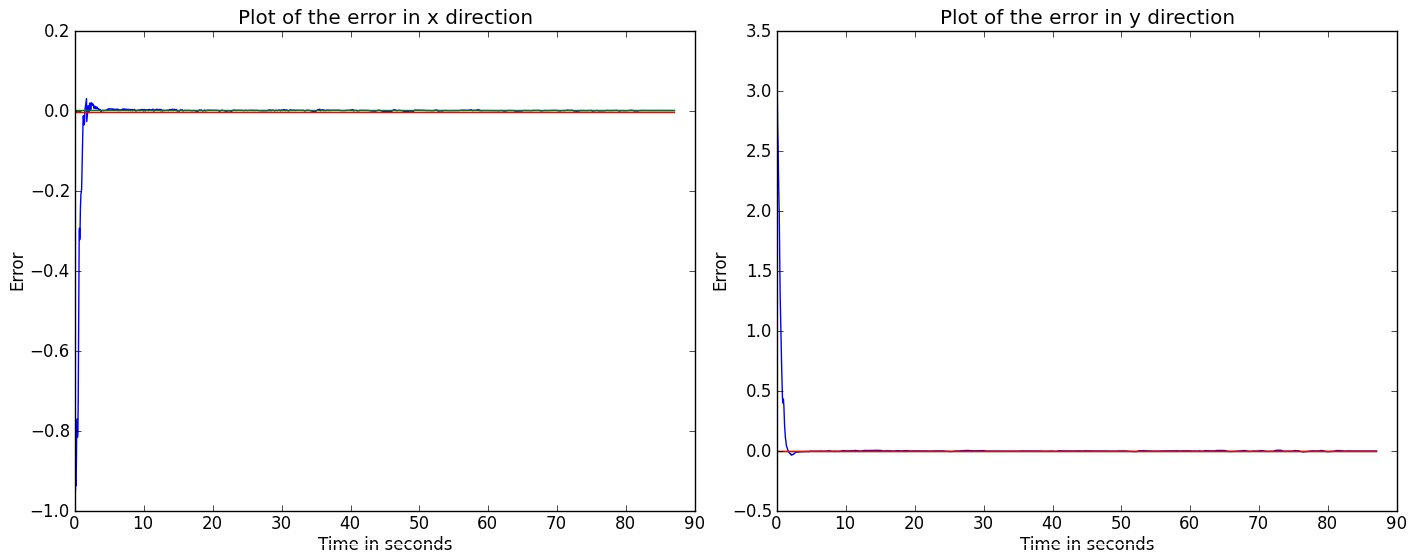
\includegraphics[width=\linewidth]{pics/startupError.jpg}
	\label{fig:startup_error_plot}
	\caption{The startup error (needs new plot!)}
\end{figure} 
As the script runs the first measurements of TimeTaken are relative big in some cases even a factor 100 from the normal values as seen in Figure ~\ref{fig:startup_error_plot} . This big value will change the angles in such a way the robot will overshoot and possibly even fall.
Therefore disregarding these values will be necessary, adding a low-pass filter to $\nabla TimeTaken$ allows finding these measurements. When the threshold of the low-pass filter has been exceeded the angle offsets will be set to 0, ignoring the large values.
\[
  Offset Hip Pitch = \left\{ 
  \begin{array}{l l}
     P_{out}x + D_{out}x& \quad \text{if $\nabla TimeTaken < Thres_{low-pass}$}\\ 
    0 & \quad \text{Otherwise}\\
  \end{array} \right.
\]

\[
  Offset Hip Roll = \left\{ 
  \begin{array}{l l}
     P_{out}y + D_{out}y& \quad \text{if $\nabla TimeTaken < Thres_{low-pass}$}\\ 
    0 & \quad \text{Otherwise}\\
  \end{array} \right.
\]
Where $Thres_{low-pass}$ is the threshold value for the low-pass filter.

\subsection{Manual tuning  (weet nog niet of dit erin moet)}

The parameters\\\\
Increasing $s$ will cause blablabla\\
$K_p$\\
$K_d$\\
$Thres_{max X}$\\
$Thres_{max Y}$\\
$Thres_{low-pass}$

\subsection{Results}

*picture from a Nao pushing the balancing Nao (the test environment)*\\\\
*plot with balancer off*\\\\
*plot with balancer on*

\subsection{The kinematics problem}
We want to be able to specify a location for the foot, then have the foot
automatically move there, which means that the we'll need to be able calculate
the required joint angles. This is known as \emph{inverse kinematics}. There is
a number of potential solutions to this problem, for example: 
\begin{itemize}
\item analytically solve the inverse kinematics chain using goniometry (as done by \cite{Graf2009})
\item use a hillclimbing algorithm to approach the desired location over a number of iterations
\end{itemize}

We wound up going with an iterative, Jacobian-based solution as decribed by
\cite{Meredith2004} and \cite{Buss2009}.

\subsubsection{Problem specification and terminology}
Let:
\begin{itemize}
    \item $\theta$ be a $1 \times n$ vector describing the angles of $n$ joints
        ($\theta = \bvect{\theta_1 & \dots & \theta_n}^T$)
    \item $\vec{t}$ the vector containing the goal position for each end effector
    \item $\vec{s}$ the vector of the end effectors' current positions
\end{itemize}

$\vec{t}$ and $\vec{s}$ are both of size $1 \times f$ where $f$ is the desired
amount of degrees of freedom in the end effectors (generally 3 if you only care
about the spatial location, or 6 if you take the rotation into account too).
Thus, if you have $k$ end effectors and 3 degrees of freedom in your position:

\begin{align*}
    \vec{t} &= \bvect{t_1, &\dots, &t_k}^T \\
    \vec{s} &= \bvect{s_1, &\dots, &s_k}^T
\end{align*}
where
\begin{align*}
    t_i &= \bvect{t_{i_{x}}, &t_{i_{y}}, &t_{i_{z}}}^T \\
    s_i &= \bvect{s_{i_{x}}, &s_{i_{y}}, &s_{i_{z}}}^T
\end{align*}

\subsection{The Kick}
With the solutions to the previous aspects of the dynamic kick constructed, 
we can start to calculate the optimal kicking trajectory. This kick is composed
of different stages, loosely based on the approach of \cite{Xu2010}. 
\begin{itemize}
    \item Initial pose
    \item Retraction point
    \item Contact point
    \item Fitting a Bezier curve
\end{itemize}

For all these stages we assume we have knowledge about the coordinates of the
ball in some coordinate system relative to the Nao or a fixed point in space,
the size of the ball to hit and which way we want to kick the ball.

\subsubsection{Initial pose}
The first stage is the initial pose. The Nao is positions its center of mass on
top of its standing leg and lowers his center of mass so as to get a more stable
position while performing his kick. This stage still makes use of the  keyvalues as 
it makes for a smoother transition to the kicking motion, without having to rely on 
the balance controllers from the start. 

\subsubsection{Contact point}
The contact point is the point on the ball that has to be hit by the Nao to
move it in the desired direction. \cite{Xu2010} uses the following
calculationt to find this, which seems to work exactly as we would like:
\begin{align*}
    \vec{c} - ( \vec{e} * r )
\end{align*}
where $\vec{c}$is the location of the center of mass of the ball, $r$ is the
ball radius(in the case of the SPL balls this is 33.42 mm) and $\vec{e}$ is the
force destination (the direction of where we want the ball to end up in
coordinates).


\subsubsection{Retraction point}
After the initial pose the Nao calculates its optimal retraction point. This
is the rearmost point from which the kick commences, and has two criteria that
should be satisfied to be considered a good starting position:
\begin{itemize}
    \item The retraction point should be far away from the ball (to make the
        kick as hard as possible)
    \item The retraction point should be accurate 
\end{itemize}
To meet both criteria as good as possible there should be a trade off between
the two.

Firstly, to determine the point between the ball and a possible retraction point
we use the following calculation: 

\begin{align*}
    d_r = ||\vec{p_{c}^{xy}} - \vec{p^{xy}} || * 0.7 + ||\vec{p_{c}^z} - \vec{p^z}|| * 0.3
\end{align*}

Where $\vec{pc}$ is the contact pointwhere the ball should be hit and
$\vec{p}$ is a possible retraction point and $\vec{d_r}$ the distance between both
points. The reason the ${xy}$ dimensions get more weight is because heightening
the feet for a bigger distance of the retraction is less desirable as it creates
more imbalance and takes up more time. The retraction n the x and y direction
however enable a more accurate and harder kick.

\begin{figure}
    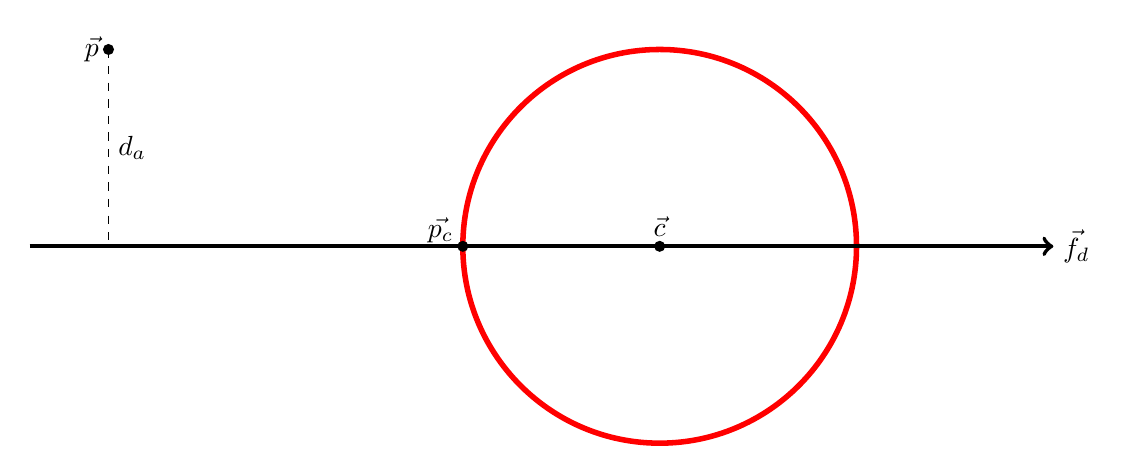
\begin{tikzpicture}
        \coordinate [label=left:$\vec{p_c}$] (A) at (-2.5,0.2);
        \coordinate [label=right:$\vec{f_d}$] (B) at (5, 0 );
        \coordinate [label=right:$d_a$] (F) at (-7, 1.25);
        \coordinate [label=above:$\vec{c}$](C) at (0,0);
        \coordinate (D) at (-2.5, 0);
        \coordinate [label=left:$\vec{p}$] (E) at (-7, 2.5);
        \draw[line width = 2][color = red] (0,0) circle (2.5cm);
        \draw [style = thick][line width = 1.5][->](-8, 0) -- (B);
        \draw[dashed] (E) -- (-7,0);
        \foreach \point in {C,D,E}
        \fill [black,opacity=1] (\point) circle (2pt);
    \end{tikzpicture}
    \caption{Visualisation of the accuracy problem. \small{the contact point
            ($\vec{p_c}$) and the preferable force direction ($\vec{f_d}$) form a line
    in 3D space. A possible retraction point $\vec{p}$ can be somewhere around
    this line. To find its accuracy the distance $d_a$ should be solved. Note that
    this only concerns the x and y direction as the z dimension does not
    influence the accuracy. $\vec{c}$ denotes the center of mass
    location on the ball and is only shown for clarification.}}
    \label{fig:accuracy}
\end{figure}    

Finding the accuracy of a given retraction point is less straightforward. This
problem can be seen as the closeness of a given point to the line, where the
point consists of a possible retraction point and the line consits of the
contact point and the destination point. See Figure \ref{fig:accuracy} for a
visualisation of the problem. This idea makes for a basic linear algebra
\footnote{The intuition behind this calculation can be found on http://mathworld.wolfram.com/Point-LineDistance3-Dimensional.html }
problem that needs to be resolved.
\begin{align*}
    d_a = \frac{(||(\vec{p^{xy}} - p_c^{xy}) \times (\vec{p^{xy}} -
    \vec{f_d})||}{\|\vec{f_d^{xy}}- \vec{p_c^{xy}}\|}
\end{align*}

The distance to the line is only important in the $xy$ direction, but a cross
product can only be taken in 3d space so this is solved by taking the $xy$
values from the original points in space but adding a 0 value in the z
direction.
Now that we have a way to calculate both the distance to the contact point and
the accuracy towards the force direction, we are able to make a balanced
decision towards what a good retraction point is.

\begin{align*}
    \vec{p} = 0.1 * d_r + 0.9 * \frac{0.1}{d_a}
\end{align*}

We take the multiplicative inverse of $d_a$ so that the value gets bigger when the
retraction point is close to the line and rescale it by deviding it with 10 to
make the value $d_r$ and $d_a$ more in the same range. The multiplicative values
0.1 and 0.9 could be experimented with to find the optimal result. In the above
equation accuracy is more important than a big distance between ball and
retraction point.

All possible positions $\vec{p}$ should be considerd to solve this equation. To
determine what is possible the Nao is set in different positions and using a
forward kinematics chain the end effector of each leg in world space coordinates
can be retrieved. This way roughly all possible positions are set and can be
looped thorugh to find the point that maximizes above equation. By also
retrieving the location of the standing leg we make sure that there is
no overlap in the reachable space and the position of the other leg.

\subsubsection{Making a kick using the Bezier curve}
now that we have 2 points which the Nao should use in space to place a kick,
making a kick withou

\section{Experiments and Results}
\subsection{Center of mass balancing}
\begin{figure}[htb]
  \centering
  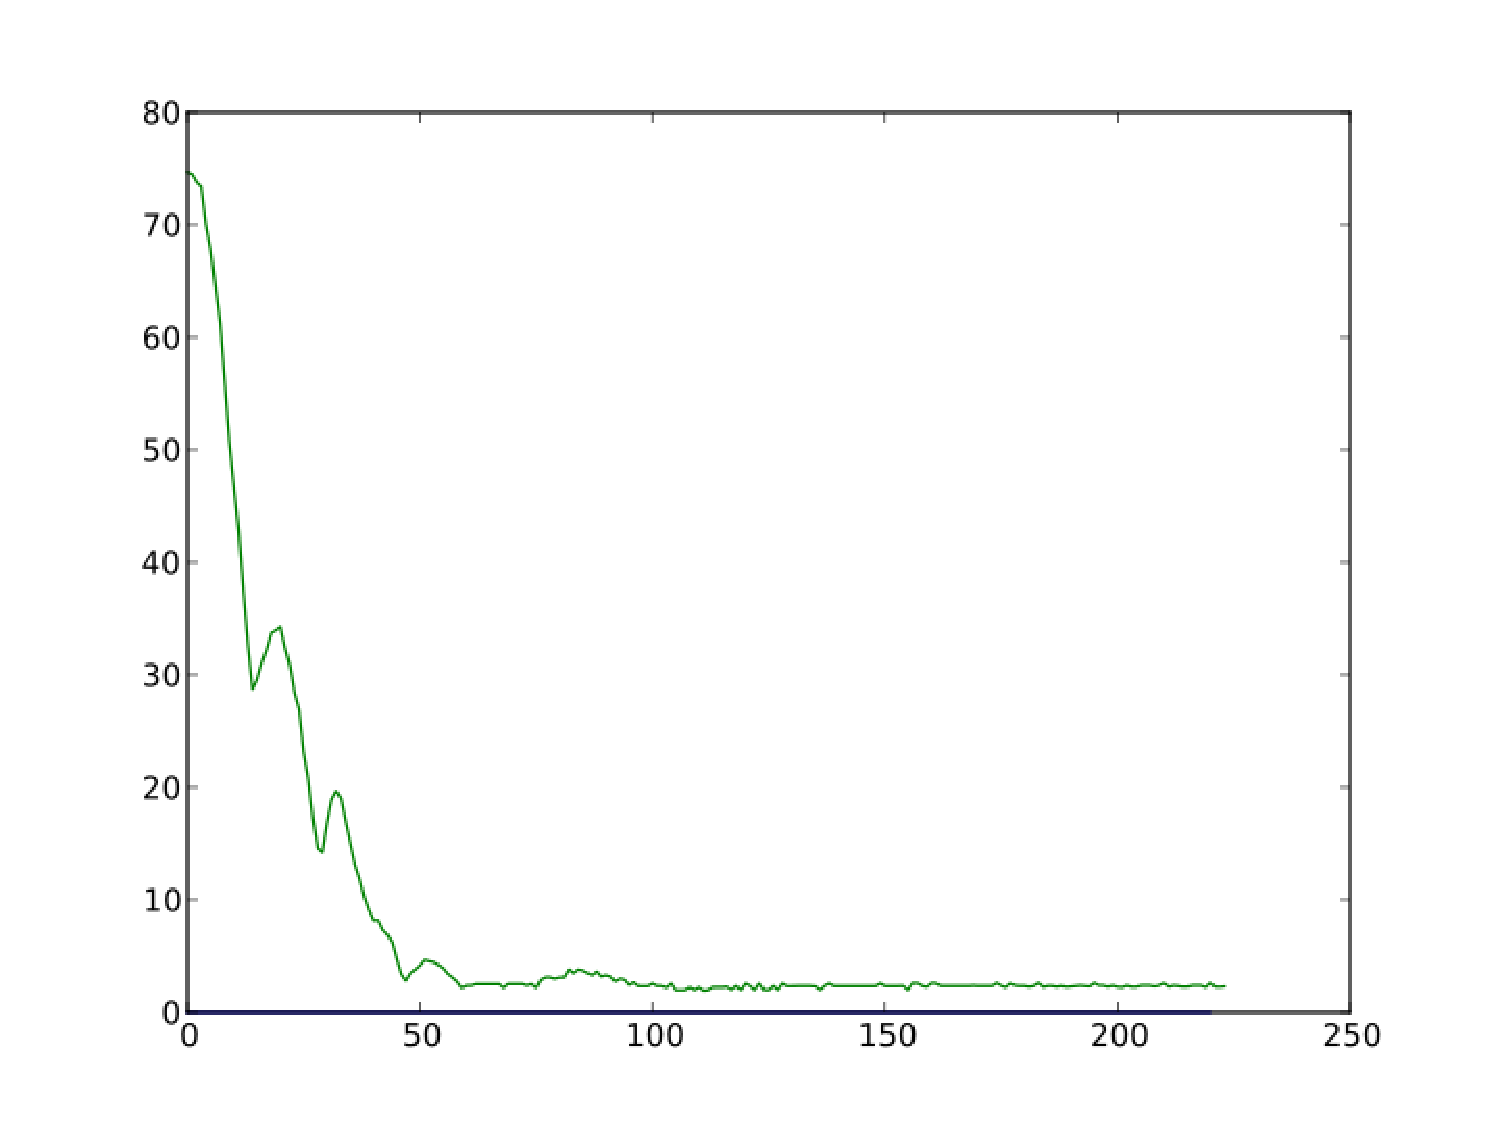
\includegraphics[width=1\textwidth]{pics/com_error__threshold_3__gain_0_0005.pdf}
  \label{fig:com_plot}
  \caption{The error of the CoM P-Controller over a number of trials}
\end{figure}

Figure \ref{fig:com_plot} shows the error of the CoM P-Controller over roughly 200
trials.

\section{Required materials and support} 
To find a solution to our problem statement we need a Nao to experiment on and a
possible simulation environment for at home. All of these materials are
available in the robolab.

Furthermore, there are different papers concerned with the problems we are
trying to tackle, but none of them cover the whole problem statement, and not
all are specifically about the Nao. For example we found a paper about
calculating the center of mass for robots with multiple joints\cite{Cotton2008} but not tailored
to the connection of joints of a  Nao robot.The difficulty for us is to put all this
information together and to make it work specifically on the Nao, and to
document this process at the same time. Most of the problems have been covered
in previous courses, but it still will require some insight in achieving our set
goals.

\section{Conclusion}
\begin{itemize}
    \item our kick is awesome
    \item using iterative inverse kinematics solutions are problematic in
        accuracy and sustainability
\end{itemize}

\section{Discussion}
Although the problem of making a dynamic kick has been solved by various teams
in the Standard Platform League already (citations, citations), there are various solutions to our
problems that we have not yet encountered in other papers. For instance the idea
of making a proportinal controller based on the Center of Mass is one that is
implemeneted often, but making a search space through which to find the optimal
position is not one we have encountered but works great.

It comes to show that although our problem initially looked as if it would be a
straight path we have been able to give it our own interpretation which only
gives the 

\section{Future works}
Now that all sub problems of making a dynamic kick are mostly succesfully
solved, there are still some future improvements we would like to work on.

\subsection{Wrapping up our current progress}
Firstly we would like to integrate all elements to make a succesful kick. This
was something we wanted to complete by the time this project ended, but in
hindsight was a little too advanced to actually complete in the limited
tiemframe. However, as we still were able to find
solutions to each and every problem (except for the inverse kinematics solver
which seems a little too unreliable) we could now take the time to put everything
together for delivering a robust kick.

\subsection{optimizing the code to run in C++}
Another future improvement is dealing with the slowness of the current
implementations for some of the calculations. For instance, making hundred
iterations with our current Inverse Kinematics solver can cost multiple seconds.
This is not an option when the Nao has to perform a kik in a Robocup match. This
can be easily solved by rewriting all our code into c++ instead of python (the
language we use now). This will surely increase the speed of our program, but if
it is fast enough remains to be seen.


As of now the code has only been tested while running from our computers, but
for the Robocup competiton it will need to run on the Naos itself.

Finally, if our kick seems to be sufficiently working we can integrate it as a
module into the current Dutch Nao Team code as to replace the hardcoded kicks.

    \item using Denavit Hartenberg for the forward kinematics
    \item making the code run on the Nao(talk about stable runningspeed which
        Richard made)
    \item Now that we have the basics we can start working on a dynamic walk
\end{itemize}

\bibliographystyle{plain}
\bibliography{library}
\end{document}
